\section{L-system grammars}

\section{D0L System}

\section{Basic 2D L-systems} 

There are a number of fractal geometry that have become well known particularly with regards to how they can seemingly imitate nature \cite{mandelbrot1982fractal}. Particularly with the geometry such as the Koch snowflake which can be represented using the following L-system.

\begin{figure}[htbp]
	\raggedright
	\textbf{\underline{Koch Curve:}} \\
	\textbf{Alphabet:} F \\
	\textbf{Constants:} +, - \\
	\textbf{Axiom:} F \\
	\textbf{Angle:} 90$^\circ$ \\
	\textbf{Rules:} \\
	F $\rightarrow$ F+F--F+F\\
	{\centering
		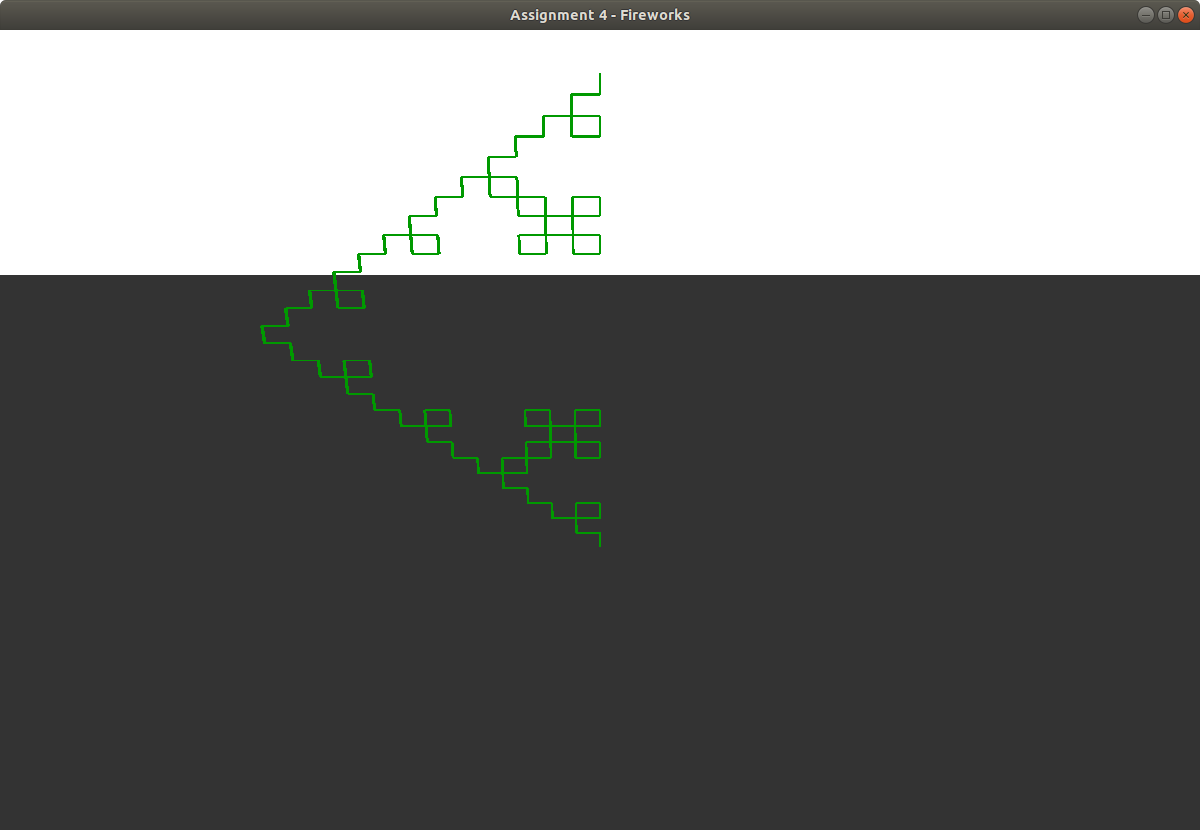
\includegraphics[scale=0.8]{KochCurve/KochCurve04.png}
		\caption{Koch Curve.}
	}
\end{figure}
\begin{figure}[htbp]
	\raggedright
	\textbf{\underline{Sierpinski Triangle:}} \\
	\textbf{Alphabet:} A, B \\
	\textbf{Constants:} +, - \\
	\textbf{Axiom:} A \\
	\textbf{Angle:} 60$^\circ$ \\
	\textbf{Rules:} \\
	A $\rightarrow$  B-A-B \\
	B $\rightarrow$ A+B+A\\
	{\centering
		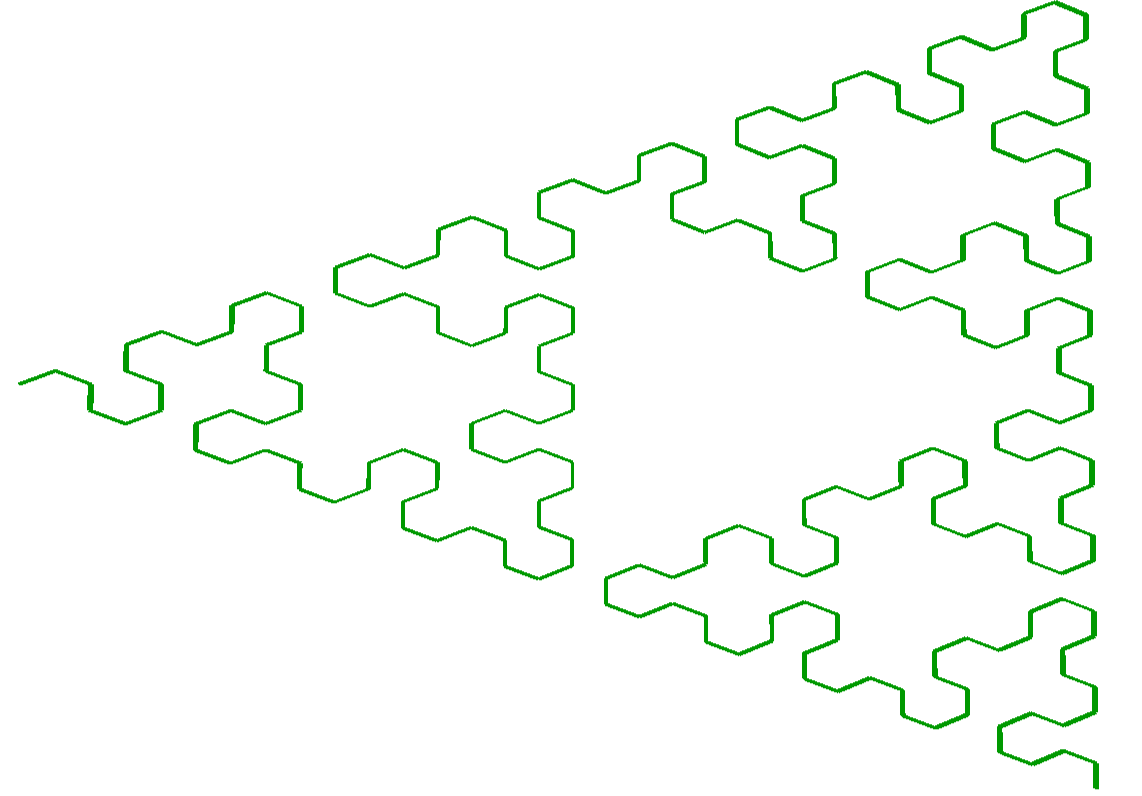
\includegraphics[scale=0.2]{SierpinskiTriangle/SierpinskiTriangle06.png}
		\caption{Sierpinski Triangle.}
	}
\end{figure}
\begin{figure}[htbp]
	\raggedright
	\textbf{\underline{Dragon Curve:}} \\
	\textbf{Alphabet:} F, X, Y \\
	\textbf{Constants:} +, - \\
	\textbf{Axiom:} FX \\
	\textbf{Angle:} 90$^\circ$ \\
	\textbf{Rules:} \\
	X $\rightarrow$ X+YF+ \\
	Y $\rightarrow$ -FX-Y\\
	{\centering
		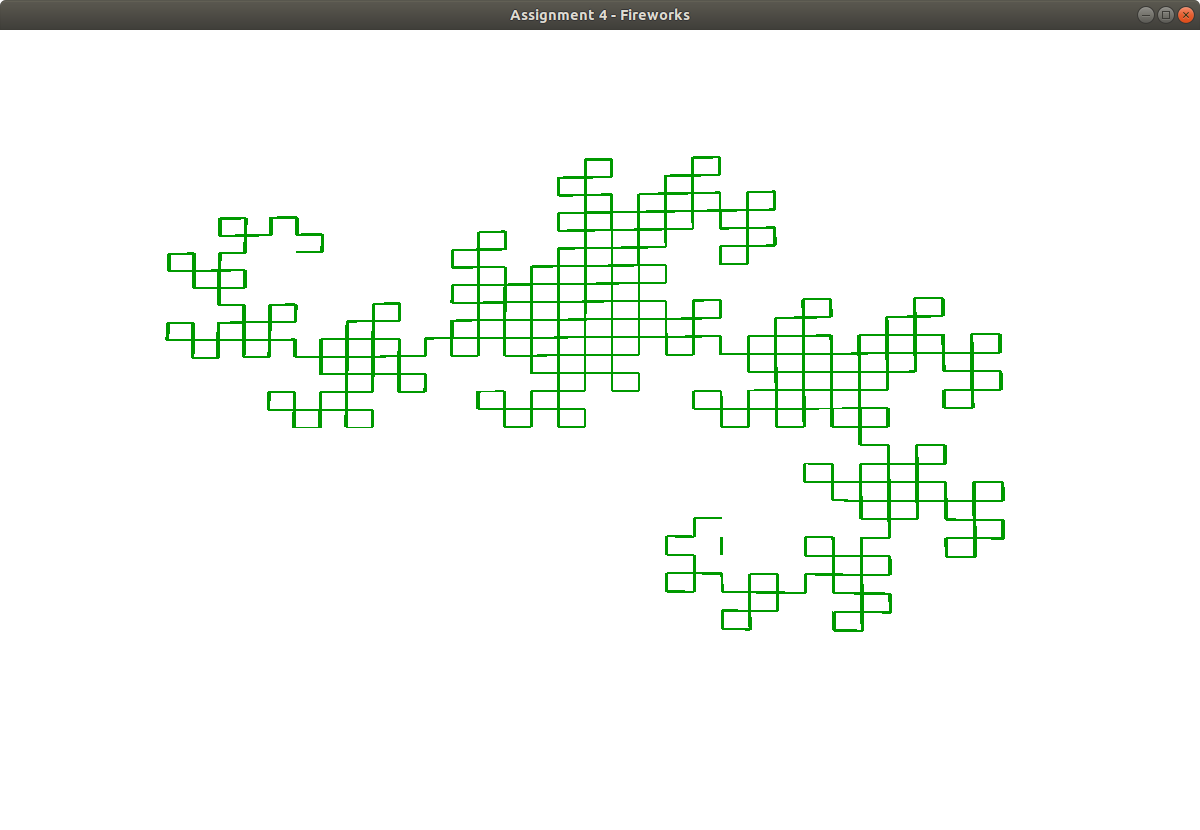
\includegraphics[scale=0.2]{DragonCurve/DragonCurve10.png}
		\caption{Dragon Curve.}
	}
\end{figure}
\begin{figure}[htbp]
	\raggedright
	\textbf{\underline{Fractal Plant:}} \\
	\textbf{Alphabet:} X, F\\
	\textbf{Constants:} +, -, [, ] \\
	\textbf{Axiom:} X \\
	\textbf{Angle:} 25$^\circ$ \\
	\textbf{Rules:} \\
	X $\rightarrow$ F-[[X]+X]+F[+FX]-X\\
	F $\rightarrow$ FF \\
	{\centering
		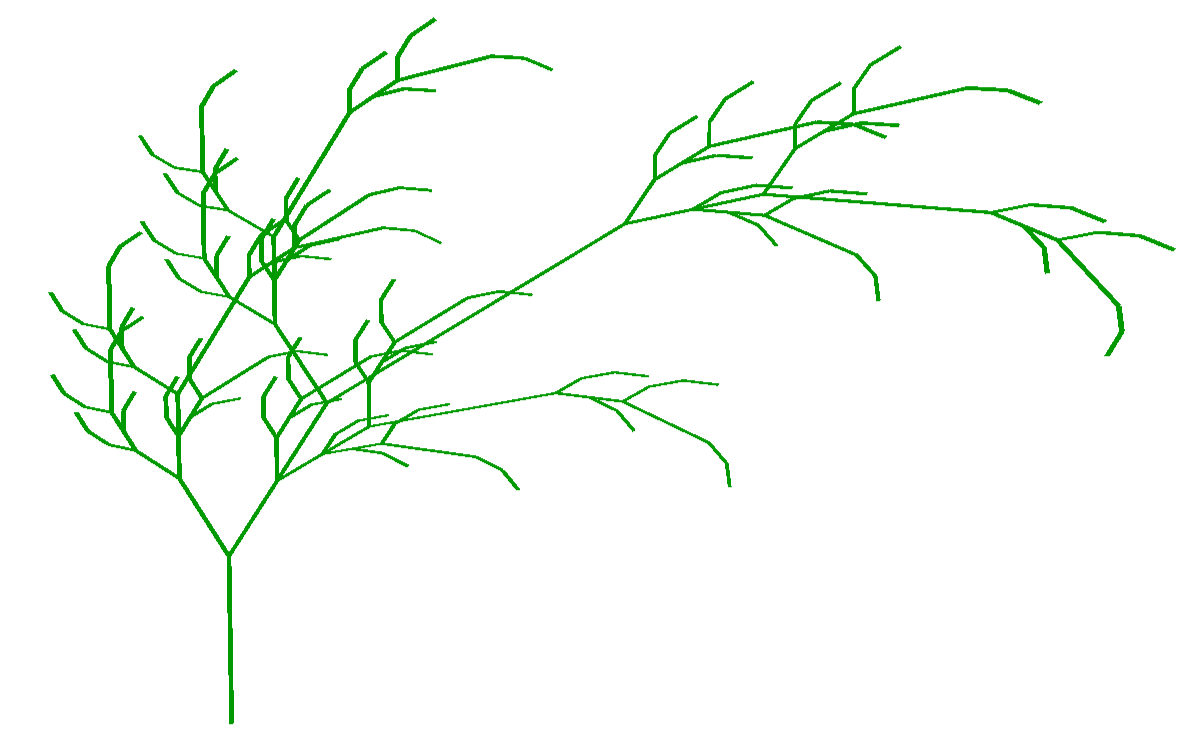
\includegraphics[scale=0.15]{FractalPlant/FractalPlant05.png}
		\caption{Fractal Plant.}
	}
\end{figure}
\begin{figure}[htbp]
	\raggedright
	\textbf{\underline{Fractal Bush:}} \\
	\textbf{Alphabet:} F\\
	\textbf{Constants:} +, -, [, ] \\
	\textbf{Axiom:} F \\
	\textbf{Angle:} 25$^\circ$ \\
	\textbf{Rules:} \\
	F $\rightarrow$ FF+[+F-F-F]-[-F+F+F]\\
	{\centering
		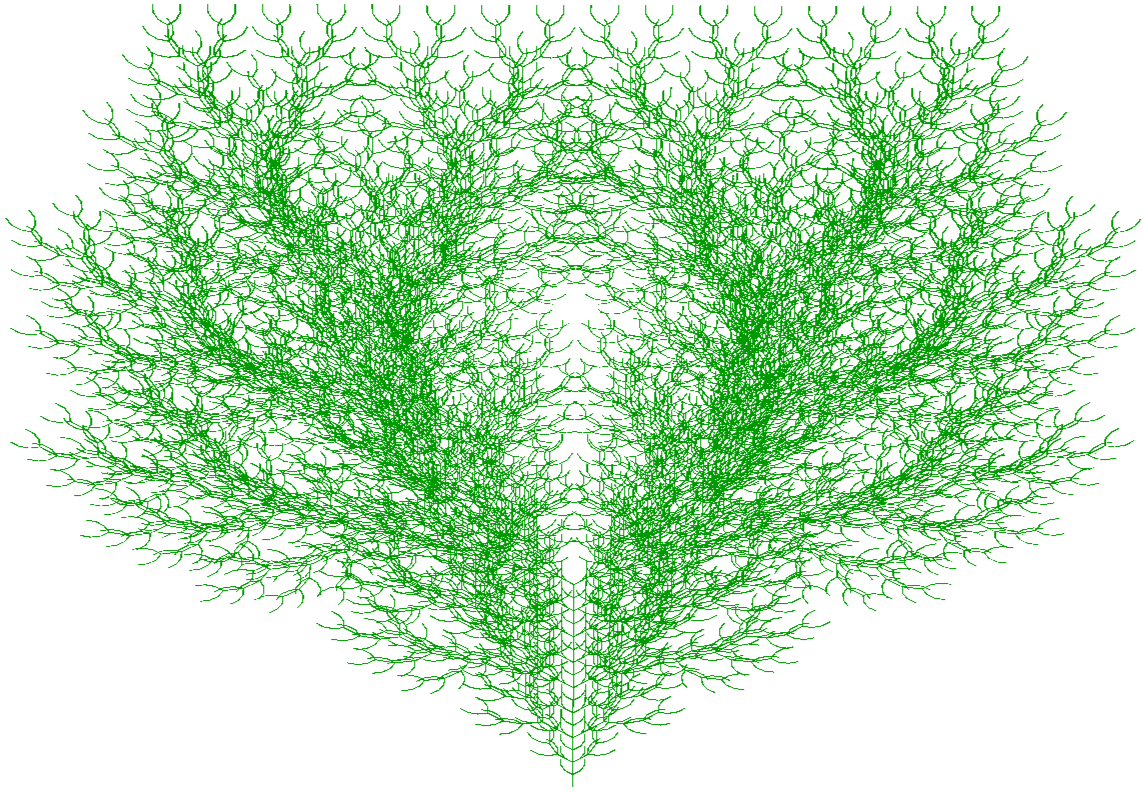
\includegraphics[scale=0.15]{FractalBush/FractalBush06.png}
		\caption{Fractal Bush.}
	}
\end{figure}

\FloatBarrier
\newpage
\section{Branching Filaments}